% Source for the public JIT multi-token vault working paper.
\documentclass[11pt]{article}

\usepackage[T1]{fontenc}
\usepackage[utf8]{inputenc}
\usepackage{lmodern}
\usepackage[margin=1in]{geometry}
\usepackage{microtype}
\usepackage{amsmath,amssymb,mathtools}
\usepackage{booktabs,tabularx,array}
\usepackage{enumitem}
\usepackage{xcolor}
\usepackage{tikz}
\usetikzlibrary{arrows.meta,positioning,shapes.geometric,fit}
\usepackage{fancyhdr}
\usepackage{hyperref}
\usepackage{cleveref}

\definecolor{sclgold}{HTML}{8B6914}
\definecolor{sclcream}{HTML}{F5F0E8}
\definecolor{sclink}{HTML}{1F2937}
\definecolor{sclmuted}{HTML}{6B6560}
\hypersetup{
  colorlinks=true,
  linkcolor=sclgold,
  citecolor=sclgold,
  urlcolor=sclgold,
  pdftitle={Just-in-Time Multi-Asset Liquidity Vaults},
  pdfauthor={Lars Fritz}
}

\pagestyle{fancy}
\fancyhf{}
\fancyhead[L]{\small\textcolor{sclmuted}{Spherical Cow Labs}}
\fancyhead[R]{\small\textcolor{sclmuted}{JIT Multi-Asset Liquidity Vaults}}
\fancyfoot[C]{\thepage}
\renewcommand{\headrulewidth}{0.3pt}
\setlength{\headheight}{14pt}
\setlist{nosep,leftmargin=1.6em}

\newcommand{\protocol}{\textsc{JIT Vault}}
\newcommand{\nav}{\mathrm{NAV}}
\newcommand{\twap}{\mathrm{TWAP}}
\newcommand{\bps}{\mathrm{bps}}
\newcommand{\E}{\mathbb{E}}
\newcommand{\R}{\mathbb{R}}

\title{\vspace{-1.5em}\textbf{Just-in-Time Multi-Asset Liquidity Vaults}\\
\large A Fund-Like AMM with Atomic Pairwise Concentrated Liquidity}
\author{Lars Fritz\\\small Spherical Cow Labs\\\small \href{mailto:lars@sphericalcowlabs.xyz}{lars@sphericalcowlabs.xyz}}
\date{August 20, 2026\\\small Working paper -- Version 0.1}

\begin{document}
\maketitle

\begin{abstract}
We propose a multi-asset automated market maker in which capital is held by a
single fund-like vault and projected into pairwise concentrated-liquidity
positions only for the duration of a swap. For three assets $X$, $Y$, and $Z$,
three Uniswap-style pools retain minimal permanent liquidity and share a
mandatory Uniswap v4 hook. When a trade arrives, a coordinator atomically
creates temporary positions in the requested pair, executes the swap, removes
the positions, and returns the residual inventory and fees to the vault.

The vault issues fungible shares. Deposits may be made in any supported token
and are converted into shares at an oracle-determined net asset value;
withdrawals are strictly in-kind in the current portfolio composition. The
temporary execution range responds to relative volatility and inventory
imbalance. We introduce a two-wing construction: one position below and one
above the reference price. The wing funded by a scarce token is widened, which
reduces near-price depth and conserves that token, while the wing funded by the
abundant token is narrowed, increasing depth in the direction that replenishes
the scarce asset. This architecture replaces multidimensional tick accounting
with ordinary pairwise concentrated-liquidity math while retaining shared
capital across all pairs. We formalize share accounting, range selection,
atomic settlement, security constraints, and a research agenda for evaluating
liquidity refresh, cross-pair order flow, and adverse selection.
\end{abstract}

\vspace{0.5em}
\noindent\textbf{Status.} This document specifies a proposed mechanism. A
Foundry proof of concept implements proportional and oracle-valued single-token
deposits, in-kind withdrawals, mandatory hook routing, adapter-supplied relative
volatility, inventory-responsive asymmetric wings, and atomic
add--swap--remove execution. A production v3 TWAP and realized-volatility
adapter remains future work. Nothing in this paper should be interpreted as
audited or production-ready software.

\tableofcontents
\newpage

\section{Introduction}

Concentrated-liquidity automated market makers allow a liquidity provider to
allocate capital to a bounded price interval rather than across the entire
positive price line. This increases marginal depth near the selected price but
requires active range management and fragments capital across pools and
positions. Multi-token pools address fragmentation by placing several assets
under one invariant, but extending concentrated liquidity to a multidimensional
tick grid introduces difficult geometric and accounting problems.

This paper takes a different route. Instead of representing one persistent
multi-asset position on a multidimensional surface, it stores the assets in a
shared vault and creates conventional two-token positions just in time. The
positions are transaction-local; the vault is persistent. For $N$ assets, the
vault can support up to $N(N-1)/2$ pair pools, while every depositor owns the
same pro-rata claim on the combined inventory.

The architecture is especially natural for a fund of correlated assets. As an
example, consider tokenized claims on technology stocks. A large common market
factor can make each stock volatile in isolation while the relative price of
two constituents remains substantially less volatile. The vault can therefore
provide narrow and deep relative-value liquidity while retaining the ability to
activate the same inventory against different constituents from one trade to
the next.

The principal contributions are:

\begin{enumerate}
  \item a fund-share model permitting deposits in any supported token and
        in-kind basket withdrawals;
  \item an atomic mint--swap--withdraw lifecycle built from ordinary
        concentrated-liquidity positions and a mandatory v4 hook;
  \item a volatility-aware range rule based on time-weighted tick observations;
  \item a two-position, inventory-asymmetric range construction;
  \item explicit treatment of liquidity refresh, cross-pair ordering, oracle
        risk, and dilution resistance; and
  \item a separation between the economic specification and the present smart
        contract proof of concept.
\end{enumerate}

\section{Background}

\subsection{Concentrated liquidity}

Let token $0$ and token $1$ have pool price $P$, measured as units of token $1$
per unit of token $0$, and let $s=\sqrt{P}$. A concentrated-liquidity position
with liquidity $L$ and bounds $P_a<P_b$ holds, while active,
\begin{align}
  x_0 &= L\left(\frac{1}{s}-\frac{1}{\sqrt{P_b}}\right), \\
  x_1 &= L\left(s-\sqrt{P_a}\right).
  \label{eq:amounts}
\end{align}
The maximum liquidity supported by token amounts $x_0,x_1$ at the current price
is therefore
\begin{equation}
L=\min\left\{
\frac{x_0}{1/s-1/\sqrt{P_b}},
\frac{x_1}{s-\sqrt{P_a}}
\right\}.
\label{eq:maxliq}
\end{equation}
Narrowing the interval increases $L$ for fixed capital, raising near-price
depth but reducing the distance to exhaustion. Widening does the opposite.

For a token-$0$ exact-input swap that remains within one active range and
ignores fees for exposition,
\begin{align}
  s' &= \frac{Ls}{L+\Delta x_0 s}, \\
  \Delta x_1^{\mathrm{out}} &= L(s-s').
  \label{eq:swap0}
\end{align}
For token $1$ into token $0$,
\begin{align}
  s' &= s+\frac{\Delta x_1}{L}, \\
  \Delta x_0^{\mathrm{out}} &= L\left(\frac{1}{s}-\frac{1}{s'}\right).
  \label{eq:swap1}
\end{align}
These are the execution primitives reused by the proposed vault.

\subsection{Hooks and atomic accounting}

Uniswap v4 places pools in a singleton \texttt{PoolManager} and permits an
external hook contract to execute at selected lifecycle points. A pool has one
hook, while one hook may serve many pools \cite{univ4hooks}. Flash accounting
allows several balance-changing operations to be netted inside one unlock
cycle, with only final currency deltas settled \cite{univ4whitepaper}. These
properties permit an atomic sequence of liquidity addition, swap, liquidity
removal, fee collection, and final settlement.

V4 does not include a built-in price oracle. A deployment that wishes to use
Uniswap-style observations must either implement observation accounting in its
hook or read a separate, sufficiently liquid v3 reference pool. V3 pools expose
historical tick and liquidity accumulators through \texttt{observe}, enabling a
geometric time-weighted average price \cite{univ3oracle,univ3whitepaper}. This
distinction is material: the minimal-liquidity execution pools proposed here
must not be treated as robust external price authorities merely because they
always have a defined spot price.

\section{System Architecture}

For three supported assets, the system contains one vault, three execution
pools, one hook, and one coordinator. The assets spend nearly all time in the
vault. Minimal protocol-owned full-range positions may remain in the pair pools
to preserve initialized pool state.

\begin{figure}[ht]
\centering
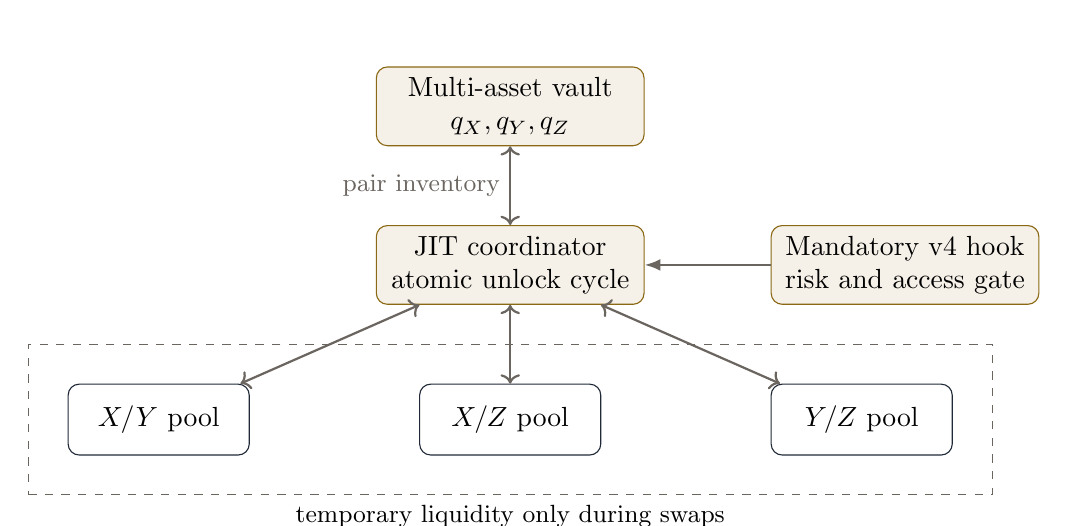
\begin{tikzpicture}[
  node distance=10mm and 16mm,
  box/.style={draw=sclgold,rounded corners,fill=sclcream,minimum width=34mm,minimum height=10mm,align=center},
  pool/.style={draw=sclink,rounded corners,minimum width=23mm,minimum height=9mm,align=center},
  arr/.style={-{Latex[length=2mm]},thick,sclmuted}
]
\node[box] (vault) {Multi-asset vault\\$q_X,q_Y,q_Z$};
\node[box,below=of vault] (coord) {JIT coordinator\\atomic unlock cycle};
\node[box,right=of coord] (hook) {Mandatory v4 hook\\risk and access gate};
\node[pool,below left=of coord] (xy) {$X/Y$ pool};
\node[pool,below=of coord] (xz) {$X/Z$ pool};
\node[pool,below right=of coord] (yz) {$Y/Z$ pool};
\draw[arr,<->] (vault) -- node[left,font=\small]{pair inventory} (coord);
\draw[arr] (hook) -- (coord);
\draw[arr,<->] (coord) -- (xy);
\draw[arr,<->] (coord) -- (xz);
\draw[arr,<->] (coord) -- (yz);
\node[draw=sclmuted,dashed,fit=(xy)(xz)(yz),inner sep=5mm,label=below:{\small temporary liquidity only during swaps}] {};
\end{tikzpicture}
\caption{Three-token architecture. The vault is the persistent economic
balance sheet; pair pools are transaction-local execution surfaces.}
\label{fig:architecture}
\end{figure}

The hook rejects every swap unless the approved coordinator has marked the
exact pool as active. If temporary vault liquidity cannot be created, the swap
reverts rather than falling through to the minimal permanent position. The
coordinator enforces a maximum trade size, a terminal price limit, and complete
exact-input consumption. Partial fills revert.

\section{Fund Shares and Cash Flows}

\subsection{Net asset value}

Let the vault hold quantities $q_i$ of assets $i=1,\ldots,N$. Let $p_i$ be a
robust oracle price in a common numeraire, and let $S$ be total fund-share
supply. The marked net asset value and share price are
\begin{align}
  \nav &= \sum_{i=1}^{N} q_i p_i, \\
  v &= \frac{\nav}{S}.
  \label{eq:nav}
\end{align}
Uncollected fees, temporary PoolManager credits, and protocol liabilities must
be included when they are economically attributable to shareholders. Share
operations are disabled while a swap cycle is active, so the marked balance
sheet is never observed halfway through temporary deployment.

\subsection{Deposit in any supported token}

A depositor may contribute $d_k$ units of any supported asset $k$. Its gross
numeraire value is $D=d_k p_k$. If the deposit adjustment is $a_k\in[0,1)$, the
shares minted are
\begin{equation}
  \Delta S=\frac{D(1-a_k)}{v}
  =\frac{d_k p_k(1-a_k)S}{\nav}.
  \label{eq:deposit}
\end{equation}
The adjustment is not merely protocol revenue. It protects existing holders
from oracle latency, execution costs, and a deposit that worsens portfolio
imbalance. A useful decomposition is
\begin{equation}
  a_k=a_0+a_{\mathrm{oracle}}+a_{\mathrm{imbalance}}+a_{\mathrm{size}},
  \label{eq:depositadjust}
\end{equation}
subject to a governed cap. A deposit that improves the mix may receive a lower
adjustment than one that increases an existing overweight. Negative adjustments
or explicit deposit rebates are possible but introduce a direct drain surface
and are excluded from the base design.

Single-token deposits require stronger oracle assumptions than proportional
basket deposits. The pricing observation must precede the deposit transaction
by enough time to resist same-block manipulation, remain fresh, and be
cross-checked against alternative markets or pair consistency. Deposits are
paused when reference data is stale or when pairwise prices imply an excessive
triangular discrepancy.

\subsection{Withdrawal only in the current mix}

A holder burning $s$ shares receives the same fraction of every vault asset:
\begin{equation}
  \Delta q_i=\frac{s}{S}q_i,\qquad i=1,\ldots,N.
  \label{eq:withdraw}
\end{equation}
The supply $S$ and balances $q_i$ in \cref{eq:withdraw} are sampled before the
burn. No oracle and no internal swap are needed. In-kind redemption prevents a
withdrawer from selecting the strongest constituent, externalizes no forced
sale to remaining holders, and ensures every fund share represents the same
portfolio distribution.

Minimal seed positions should be protocol-owned or funded by permanently
locked shares. Otherwise the last withdrawing holder could remove the state
intended to keep execution pools initialized.

\section{Atomic Swap Lifecycle}

For an exact-input trade from asset $i$ to asset $j$, the intended lifecycle is:

\begin{enumerate}
  \item validate the pool, token pair, oracle status, input size, and user
        minimum output;
  \item lock deposits and withdrawals and lend the vault's $i/j$ inventory to
        the coordinator;
  \item read the canonical reference price, volatility, and current portfolio
        weights;
  \item construct the lower and upper temporary positions described in
        \cref{sec:ranges};
  \item add both positions in one PoolManager unlock cycle;
  \item execute the user swap with a protocol-defined terminal price limit;
  \item require the exact input to be fully consumed;
  \item remove both positions and collect principal and fees;
  \item settle net PoolManager deltas, pay the user, and return all residual
        pair inventory to the vault; and
  \item verify zero residual temporary liquidity, zero coordinator balances,
        vault solvency, and lock release.
\end{enumerate}

After a successful $i\rightarrow j$ swap,
\begin{equation}
  q_i'=q_i+\Delta q_i^{\mathrm{in}},\qquad
  q_j'=q_j-\Delta q_j^{\mathrm{out}},
  \label{eq:vaulttransition}
\end{equation}
with all other balances unchanged except for explicitly charged protocol fees.
The LP fee remains in the vault because the vault owned the temporary
positions.

\section{Volatility- and Inventory-Aware Ranges}
\label{sec:ranges}

\subsection{Relative volatility}

For assets $i$ and $j$ with annualized volatilities $\sigma_i,\sigma_j$ and
correlation $\rho_{ij}$, relative log-price volatility satisfies
\begin{equation}
  \sigma_{ij}=\sqrt{\sigma_i^2+\sigma_j^2-2\rho_{ij}\sigma_i\sigma_j}.
  \label{eq:relativevol}
\end{equation}
Strongly correlated constituents can therefore support tighter relative ranges
than their standalone volatility would suggest.

On chain, the strategy estimates realized relative volatility from time-weighted
tick observations. Let $\bar{t}_m$ be average ticks over equal intervals of
length $\Delta t$. Because a Uniswap tick represents $\log_{1.0001}P$, define
\begin{equation}
  r_m=\log(1.0001)(\bar{t}_m-\bar{t}_{m-1}),
\end{equation}
and an annualized estimator
\begin{equation}
  \widehat{\sigma}_{ij}=
  \sqrt{\frac{T_{\mathrm{year}}}{M\Delta t}
  \sum_{m=1}^{M}(r_m-\bar r)^2}.
  \label{eq:realizedvol}
\end{equation}
The base log half-width is
\begin{equation}
  h_{ij}^{\sigma}=\operatorname{clip}
  \left(k\widehat{\sigma}_{ij}\sqrt{\tau},h_{\min},h_{\max}\right),
  \label{eq:volwidth}
\end{equation}
where $\tau$ is the risk horizon represented by one refresh cycle and $k$ is a
governed coverage multiplier. A volatility floor prevents pathological
concentration in quiet samples; a cap prevents the vault from exposing its
entire inventory to an uninformative range after a volatility spike.

\subsection{Inventory imbalance}

Let marked portfolio weight and target weight be
\begin{equation}
  w_i=\frac{q_i p_i}{\nav},\qquad \pi_i>0,\qquad \sum_i\pi_i=1.
\end{equation}
For pair $0/1$, define relative imbalance
\begin{equation}
  m_{01}=\log\left(\frac{w_0/\pi_0}{w_1/\pi_1}\right).
  \label{eq:imbalance}
\end{equation}
Then $m_{01}<0$ means token $0$ is underrepresented relative to token $1$.

\subsection{Two one-sided positions}

Instead of one symmetric position, the coordinator creates two wings around
reference price $P^*$:
\begin{align}
  \mathcal{R}_{\downarrow} &= [P^*e^{-h_{\downarrow}},P^*],\\
  \mathcal{R}_{\uparrow} &= [P^*,P^*e^{h_{\uparrow}}].
  \label{eq:wings}
\end{align}
At $P^*$, the lower wing is funded by token $1$ and supports token $0$ input as
price moves downward. The upper wing is funded by token $0$ and supports token
$1$ input as price moves upward. In practice, the ranges overlap by at least a
small tick buffer around $P^*$ so both directions are executable despite
boundary conventions and rounding.

We propose
\begin{align}
  h_{\downarrow} &= \operatorname{clip}
  \left(h_{01}^{\sigma}e^{\lambda m_{01}},h_{\min},h_{\max}\right),\\
  h_{\uparrow} &= \operatorname{clip}
  \left(h_{01}^{\sigma}e^{-\lambda m_{01}},h_{\min},h_{\max}\right),
  \label{eq:asymwidth}
\end{align}
where $\lambda\ge 0$ controls inventory sensitivity. If token $0$ is scarce
($m_{01}<0$), the token-$0$-funded upper wing becomes wider and the
token-$1$-funded lower wing becomes narrower. For fixed inventory this has two
effects:

\begin{itemize}
  \item the scarce token $0$ is spread over a wider interval, reducing marginal
        depth for trades that remove more token $0$; and
  \item the abundant token $1$ is concentrated into a narrower interval,
        increasing depth for traders who sell token $0$ to the vault.
\end{itemize}

The resulting one-sided liquidities, prior to the small overlap adjustment, are
\begin{align}
  L_{\downarrow}
  &=\frac{y_{\downarrow}}
  {\sqrt{P^*}-\sqrt{P^*e^{-h_{\downarrow}}}},\\
  L_{\uparrow}
  &=\frac{x_{\uparrow}}
  {1/\sqrt{P^*}-1/\sqrt{P^*e^{h_{\uparrow}}}}.
  \label{eq:wingliq}
\end{align}
Range width alone does not guarantee economically desirable rebalancing.
Capital allocation, fee asymmetry, terminal price limits, and quote skew may
also be required. The proposed width rule should therefore be treated as a
transparent baseline rather than an optimum.

\begin{figure}[ht]
\centering
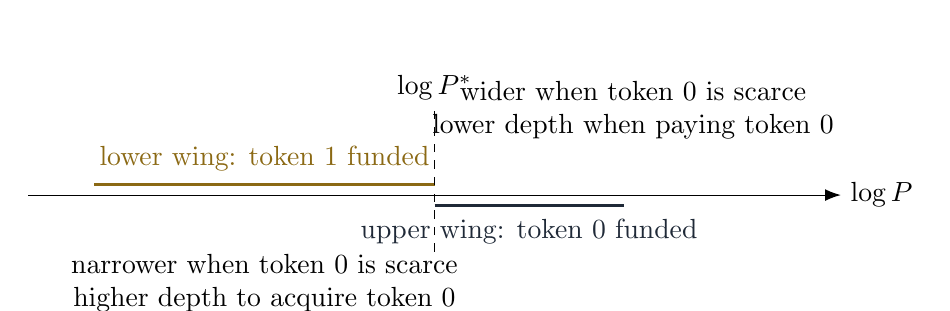
\begin{tikzpicture}[x=1.2cm,y=0.9cm]
  \draw[-{Latex[length=2mm]}] (-4.3,0) -- (4.3,0) node[right] {$\log P$};
  \draw[very thick,sclgold] (-3.6,0.15) -- (0,0.15);
  \draw[very thick,sclink] (0,-0.15) -- (2.0,-0.15);
  \draw[dashed] (0,-0.8) -- (0,1.2) node[above] {$\log P^*$};
  \node[above,text=sclgold] at (-1.8,0.2) {lower wing: token 1 funded};
  \node[below,text=sclink] at (1.0,-0.2) {upper wing: token 0 funded};
  \node[below,align=center] at (-1.8,-0.7) {narrower when token 0 is scarce\\higher depth to acquire token 0};
  \node[above,align=center] at (2.1,0.65) {wider when token 0 is scarce\\lower depth when paying token 0};
\end{tikzpicture}
\caption{Illustrative asymmetric wings when token $0$ is underrepresented.
The apparent left/right widths are schematic.}
\label{fig:wings}
\end{figure}

\section{Oracle and Price Consistency}

The system needs three distinct price concepts:

\begin{enumerate}
  \item \textbf{execution state}: the current square-root price stored by the
        selected v4 pool;
  \item \textbf{reference price}: a manipulation-resistant price used for NAV,
        deposits, volatility, and risk checks; and
  \item \textbf{strategy center}: the price around which temporary ranges are
        placed after any permitted inventory or fee skew.
\end{enumerate}

These values may be close but must not be conflated. In particular, minimal
permanent liquidity guarantees a defined execution price, not a trustworthy
reference price.

For three assets, only two pair prices are independent. With consistent units,
\begin{equation}
  P_{XZ}=P_{XY}P_{YZ}.
  \label{eq:triangle}
\end{equation}
Before minting substantial temporary liquidity, the hook should reject a pool
whose execution state deviates excessively from both the reference price and
the implied cross-price. Deposits require an even stricter oracle mode because
they mint a permanent claim on the entire vault.

An initial implementation may read deep external v3 pools and use their native
observations. A self-contained v4 implementation must add observation storage
to the hook. In both cases the policy should specify observation window,
minimum observation cardinality, minimum reference liquidity, staleness limit,
maximum cross-source deviation, and behavior during market closure or oracle
failure.

\section{Dynamic Fees and Risk Limits}

A baseline directional fee for trade $i\rightarrow j$ can be written
\begin{equation}
  f_{i\rightarrow j}=operatorname{clip}\left(
  f_0+a\widehat{\sigma}_{ij}
  +b\frac{D}{q_i p_i}
  +c\,\mathcal{T}
  +d\,\mathcal{I}_{i\rightarrow j},
  f_{\min},f_{\max}\right),
  \label{eq:fee}
\end{equation}
where $D$ is input notional, $\mathcal{T}$ measures oracle uncertainty or toxic
flow, and $\mathcal{I}_{i\rightarrow j}$ penalizes trades that worsen inventory
imbalance. Trades that improve the mix may pay a lower fee but should not
receive an unbounded rebate.

Each pool additionally requires:

\begin{itemize}
  \item a maximum input fraction of the relevant vault inventory;
  \item a maximum terminal tick movement;
  \item a user-specified minimum output;
  \item exact-input full-consumption verification;
  \item minimum and maximum allowed range widths;
  \item a pool-level pause switch; and
  \item global limits on cumulative per-block or per-epoch inventory movement.
\end{itemize}

\section{Liquidity Refresh and Cross-Pair Flow}

Removing and re-centering liquidity after every swap refreshes marginal depth.
Consequently, splitting one order into several swaps need not produce the same
output as executing it once:
\begin{equation}
  \sum_{k=1}^{n}Q_{\mathrm{refresh}}(\Delta/n)
  \ne Q_{\mathrm{single}}(\Delta).
  \label{eq:split}
\end{equation}
This is a defining feature rather than a rounding artifact. Re-centering can
increase effective liquidity, but it also repeatedly sells short-horizon
convexity to informed traders.

Shared inventory creates cross-pair state dependence. In the sequence
\begin{equation*}
  X\rightarrow Y,\qquad Z\rightarrow Y,\qquad Y\rightarrow X,
\end{equation*}
the middle trade changes the $Y$ inventory available to the final $X/Y$ range.
An attacker may therefore sandwich a victim through a different pair. Testing
only isolated pools will miss this behavior.

Three refresh policies merit comparison:

\begin{enumerate}
  \item \textbf{per-swap refresh}: every trade receives a newly constructed
        range from the latest global state;
  \item \textbf{virtual persistence}: physical positions are temporary, but
        virtual bounds and consumed depth persist until a governed rebalance;
        and
  \item \textbf{epoch clearing}: all transactions in an interval use one state
        snapshot and ranges refresh only between epochs.
\end{enumerate}

The proof of concept implements the first policy. The economically preferred
policy remains an empirical question.

\section{Security Considerations}

The architecture combines fund accounting, oracle-dependent share issuance,
temporary external liquidity, and hook-controlled swaps. The attack surface is
therefore broader than that of a passive ERC-20 vault or vanilla pool.

\subsection{Oracle-priced deposit dilution}

If $p_k$ is overstated during a single-token deposit, the depositor receives too
many shares and dilutes existing holders. Deposit pricing must use a lagged or
time-weighted observation, conservative rounding, staleness checks, and an
adjustment sufficient to cover uncertainty. A deposit should never use the
minimal execution pool's instantaneous spot price as its sole authority.

\subsection{Cross-pair and triangular extraction}

Independent pool prices can violate \cref{eq:triangle}. Deploying deep
temporary liquidity at a stale pair price turns a small discrepancy into a
large arbitrage opportunity. All pair activations must reference one canonical
price vector and globally ordered vault state.

\subsection{Reentrancy and settlement}

The hook should remain a narrow gate. A separate coordinator should own the
PoolManager unlock callback and orchestrate liquidity changes. Deposits and
withdrawals remain locked until all pair balances are returned. Postconditions
must verify zero coordinator balances, zero temporary liquidity, settled
currency deltas, non-negative vault balances, and released locks.

\subsection{Token behavior and market events}

Fee-on-transfer, rebasing, callback-bearing, paused, or blacklisting tokens can
invalidate balance-delta assumptions. The base design admits only explicitly
approved vanilla ERC-20 assets. Tokenized equities add market closures,
corporate actions, trading suspensions, dividends, splits, and issuer or
custodian risk. These are not solved by AMM mathematics and require a separate
legal and operational specification.

\subsection{Governance}

Range, oracle, fee, asset-list, and pause parameters have direct economic
effect. Production governance should use bounded parameter domains, timelocks,
role separation, emergency controls, public monitoring, and independent
security review. Uniswap's hook security guidance specifically identifies
rounding, custom math, oracle dependencies, and hook-held liquidity as areas
requiring invariant testing and specialist review \cite{univ4security}.

\section{Prototype Mapping}

The public proof of concept maps the specification into three contracts:

\begin{table}[ht]
\centering
\small
\begin{tabularx}{\textwidth}{@{}p{0.26\textwidth}X p{0.20\textwidth}@{}}
\toprule
Component & Current responsibility & Status \\
\midrule
\texttt{JITFundVault} & Holds three assets, issues proportional or
oracle-valued single-token shares, locks the balance sheet, and lends pair
inventory. & Implemented for 18-decimal assets with a freshness-checked oracle
adapter. \\
\texttt{JITSwapHook} & Rejects swaps unless an approved coordinator has an
active cycle for the exact pool. & Implemented. \\
\texttt{JITSwapCoordinator} & Computes two volatility- and inventory-sensitive
temporary wings; adds, swaps, removes, settles, and returns assets.
& Implemented; eleven end-to-end tests pass. \\
Single-token deposit & Oracle-valued share minting using
\cref{eq:deposit}. & Implemented with a governed deposit fee. \\
Oracle and volatility & Reference price, tick observations, volatility, and
cross-price validation. & Adapter interface and freshness checks implemented;
production v3 adapter and cross-price validation remain open. \\
Asymmetric wings & Two temporary positions using
\cref{eq:asymwidth,eq:wingliq}. & Implemented with governed caps, overlap, and
inventory allocation. \\
\bottomrule
\end{tabularx}
\caption{Relationship between this whitepaper and the current proof of concept.}
\label{tab:prototype}
\end{table}

The current tests cover proportional and single-token deposits, in-kind
withdrawal, atomic two-wing execution, inventory-responsive widths, inventory
return, a cross-pair sequence, direct-router rejection, trade-size limits,
terminal-tick partial-fill rejection, and removal of trader-controlled range
parameters. They do not constitute economic validation or an audit.

\section{Economic Interpretation}

The vault resembles an index fund that also operates a relative-value market
maker. Its marked return can be decomposed schematically as
\begin{equation}
  R_{\mathrm{vault}}=
  R_{\mathrm{basket}}
  +R_{\mathrm{fees}}
  +R_{\mathrm{rebalancing}}
  -R_{\mathrm{adverse\ selection}}
  -R_{\mathrm{MEV}}
  -R_{\mathrm{operations}}.
  \label{eq:return}
\end{equation}
The design does not manufacture economic capital. It increases effective local
liquidity by repeatedly concentrating existing capital at the active pair and
price. Shareholders are compensated through fees for bearing inventory risk,
relative-price risk, and adverse selection.

Correlated assets are attractive because $\sigma_{ij}$ in
\cref{eq:relativevol} may be small, but correlation is state-dependent and can
break during stress. A strategy calibrated only on quiet-period correlation is
likely to be most concentrated precisely when relative risk begins to expand.
Volatility floors, caps, rapid pause conditions, and stress testing are
therefore essential.

\section{Evaluation Plan}

A credible evaluation should compare the proposed system against independent
v3/v4 pools, a conventional managed-liquidity vault, and a multi-token
invariant. At minimum, simulations and historical replay should report:

\begin{itemize}
  \item output and price impact by trade size and direction;
  \item capital utilization and fraction of inventory activated;
  \item fee income, loss-versus-rebalancing, and marked LP P\&L;
  \item portfolio-weight deviation and time to recover from imbalance;
  \item results for one large trade versus an equivalent split order;
  \item cross-pair and triangular sandwich profitability;
  \item performance across volatility and correlation regimes;
  \item oracle-lag loss and deposit-dilution stress cases;
  \item gas cost of two temporary positions and full settlement; and
  \item failure behavior at range boundaries, token exhaustion, and market
        closure.
\end{itemize}

The test harness should fuzz globally ordered sequences rather than independent
pair calls. Formal invariants should include share non-dilution under fair
pricing, asset conservation up to bounded rounding dust, no residual temporary
liquidity, no residual coordinator balance, and solvency after every successful
operation.

\section{Open Questions}

The following questions remain deliberately unresolved:

\begin{enumerate}
  \item Should temporary ranges refresh per swap, persist virtually, or clear
        by epoch?
  \item Is the reference price best obtained from external v3 TWAPs, a custom
        v4 hook oracle, or a median of venues?
  \item How should deposit adjustments divide between existing shareholders,
        protocol reserves, and insurance?
  \item Should target weights be fixed, governance-controlled, or endogenous to
        deposits and withdrawals?
  \item Is width asymmetry sufficient, or should capital allocation, price
        center, and fees also be directionally skewed?
  \item What execution policy best limits cross-pair MEV without sacrificing
        composability?
  \item How should market hours and corporate actions be handled for tokenized
        real-world assets?
\end{enumerate}

\section{Conclusion}

The JIT multi-asset vault replaces a persistent multidimensional AMM position
with a persistent fund balance sheet and temporary pairwise execution. This
preserves familiar concentrated-liquidity mathematics, allows one inventory to
serve every supported pair, and makes all shareholders owners of the same
portfolio distribution. Single-token deposits improve accessibility, while
in-kind withdrawals keep redemption accounting simple and avoid forced sales.

Volatility-aware widths and two asymmetric wings allow execution depth to
respond to both market risk and portfolio imbalance. Yet the same mechanisms
create the central research challenges: refreshed liquidity changes order
splitting economics, shared balances connect sandwiches across pairs, and
oracle-priced deposits create a permanent dilution surface. Uniswap v4 supplies
useful atomic execution and hook primitives, but it does not remove the need for
a coherent global price vector, conservative share accounting, adversarial
economic testing, and independent audit.

\section*{Disclaimer}

This paper is for research and informational purposes only. It is not investment,
legal, tax, or accounting advice, and it does not describe an audited or
production-ready system. Tokenized securities and fund-like products may be
subject to extensive regulatory, licensing, disclosure, custody, and market
structure requirements.

{\small
\begin{thebibliography}{9}

\bibitem{univ3whitepaper}
H.~Adams, N.~Zinsmeister, M.~Salem, R.~Keefer, and D.~Robinson.
\newblock \emph{Uniswap v3 Core}.
\newblock 2021. \url{https://app.uniswap.org/whitepaper-v3.pdf}.

\bibitem{univ3oracle}
Uniswap Labs.
\newblock \emph{Price Oracles: Uniswap v3 Developer Documentation}.
\newblock \url{https://developers.uniswap.org/docs/protocols/v3/concepts/price-oracles}.

\bibitem{univ4whitepaper}
H.~Adams, N.~Zinsmeister, S.~Moody, R.~Rivera, I.~A. Salem, and M.~D. Robinson.
\newblock \emph{Uniswap v4 Core}.
\newblock 2024. \url{https://app.uniswap.org/whitepaper-v4.pdf}.

\bibitem{univ4hooks}
Uniswap Labs.
\newblock \emph{Uniswap v4 Hooks: Developer Documentation}.
\newblock \url{https://developers.uniswap.org/docs/protocols/v4/concepts/hooks}.

\bibitem{univ4security}
Uniswap Labs.
\newblock \emph{Uniswap v4 Hook Security Framework}.
\newblock \url{https://developers.uniswap.org/docs/protocols/v4/security}.

\bibitem{balancer}
F.~Martinelli and N.~Mushegian.
\newblock \emph{Balancer: A Non-Custodial Portfolio Manager, Liquidity Provider,
and Price Sensor}.
\newblock 2019. \url{https://balancer.fi/whitepaper.pdf}.

\end{thebibliography}
}

\end{document}
